\section{Grundlagen}

\subsection{Die Benutzeroberfläche}
Die folgende Abbildung zeigt die Benutzeroberfläche mit Beispieldaten.\\\\
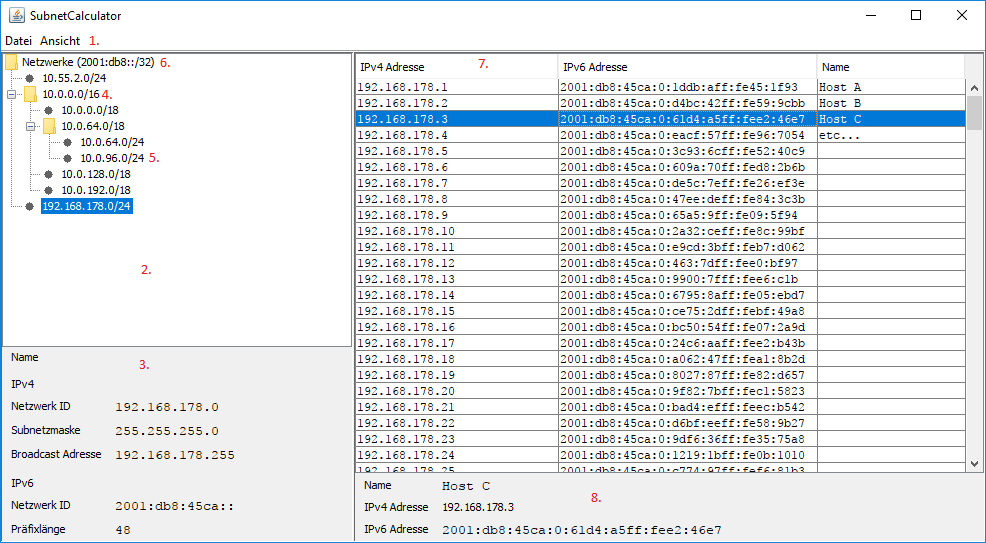
\includegraphics[width=\textwidth]{resources/oberflaeche.png}\\
\begin{enumerate}
    \item Menüleiste mit grundlegenden Funktionen
    \item Übersicht über alle Netzwerke und Subnetzwerke
    \item Details über das aktuell ausgewählte Netzwerk oder Subnetzwerke
    \item Ein Netzwerk
    \item Ein Subnetzwerk
    \item Globaler IPv6 Präfix
    \item Liste aller Hosts im aktuell ausgewählten Netzwerk
    \item Information über den aktuell ausgewählten Host
\end{enumerate}

\subsection{Funktionsweise}
Bei der Planung mit dem \subnetcalc\ werden grundlegend 3 Objekte unterschieden.

\subsubsection{Netzwerk}
Ein Netzwerk beschreibt ein Stammnetzwerk. Diese werden in der Oberfläche im
Netzwerkbaum direkt unter dem Punkt "`Netzwerke"' angezeigt.
Die Netzwerke liegen alle in einem logischen Stammnetzwerk mit der IPv4 Adresse
0.0.0.0/0. Daher dürfen sich die Netzwerke nicht überschneiden.

\subsubsection{Subnetzwerk, Subnetz}
Das Subnetzwerk, kurz Subnet, beschreibt ein Subnetzwerk eines Netzwerkes. Die
Subnetze eines Netzwerkes dürfen sich, wie die Netzwerke nicht überschneiden.
Subnetze können beliebig verschachtelt werden, wobei ein Subnetz entweder
weitere Subnetze oder Hosts enthalten darf.

Aus der technischen Sicht verhalten sich Netzwerke und Subnetzwerke gleich.
Daher wird im folgenden, wenn nicht anders beschrieben, nicht zwischen Netwerk
und Subnetzwerk unterschieden.

\subsubsection{Host}
Der Host beschreibt einen IP Endpunkt im Netzwerk, z.B. einen Computer. Hosts
liegen in einem  Netzwerk und haben immer eine zugewiesene IPv4 Adresse.
Wenn das Netzwerk mit IPv6 konfiguriert wurde, kann der Host auch eine IPv6
Adresse besitzen. Auch wenn bei der IPv6 Konfiguration in der Regel mehrere IPv6
Adressen pro Host oder Schnittstelle eingetragen werden, ist dies in dieser Software
nicht vorgesehen.

\subsection{Bedienung über das Kontextmenü}
Die meisten Bedienelemente sind in einem Kontextmenü enthalte, welches Sie über
einen Rechtsklick auf den Stammeintrag, ein Netzwerk oder ein Subnetz in der
Baumstruktur erreichen, oder auf einen Host in der Hosttabelle.